%
% schwach.tex
%
% (c) 2023 Prof Dr Andreas Müller
%
\begin{figure}
\centering
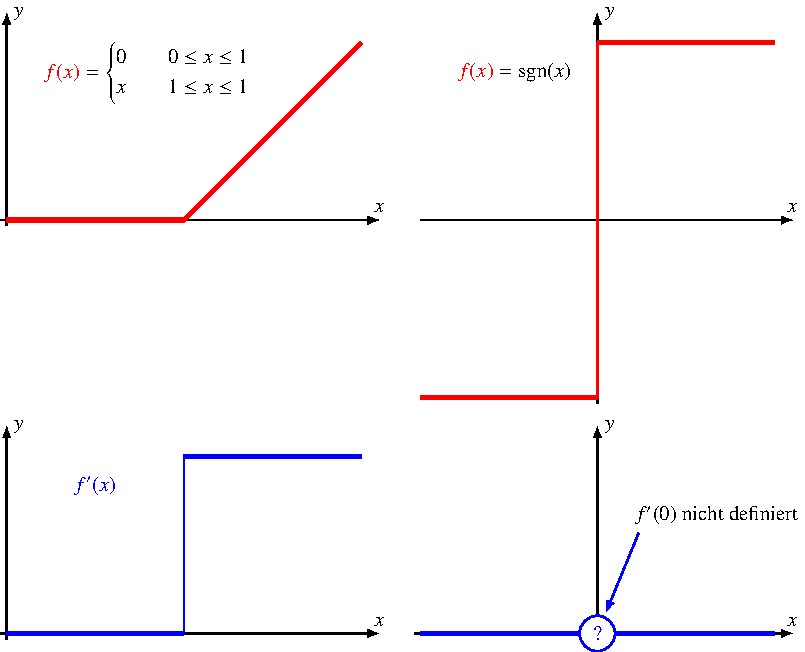
\includegraphics{chapters/010-skalarprodukt/images/schwach.pdf}
\caption{Schwache Ableitung einer nicht differenzierbaren Funktion.
Links die schwache Ableitung der Funktion von
Beispiel~\ref{buch:skalarprodukt:sobolevraum:bsp:schwachexistiert}.
Für die Signum-Funktion von
Beispiel~\ref{buch:skalarprodukt:sobolevraum:bsp:schwachexistiertnicht}
existiert die schwache Ableitung nicht, sie lässt für den Punkt $0$
nicht definieren.
\label{buch:skalarprodukt:sobolevraum:fig:schwach}}
\end{figure}
